%% This is an example first chapter.  You should put chapter/appendix that you
%% write into a separate file, and add a line \include{yourfilename} to
%% main.tex, where `yourfilename.tex' is the name of the chapter/appendix file.
%% You can process specific files by typing their names in at the
%% \files=
%% prompt when you run the file main.tex through LaTeX.

This chapter contains architectural references to concepts that research facility sites utilize to implement 5G services through network slicing. These are mainly based on \acrshort{3gpp} specifications, but also take into consideration work in other \acrshort{sdo} for vertical requirements and the 5G evolution.

\section{Network Slicing as a Concept}
5G networks, in combination with network slicing, deliver business customers connectivity and data processing tailored to the specific business requirements that adhere to a \acrfull{sla} agreed with the network operator. The customisable network capabilities include data throughput, quality, latency, reliability and security. From a mobile operator’s point of view, a network slice is an independent end-to-end logical network that runs on a shared physical infrastructure, capable of providing a negotiated service quality. 

As previously mentioned in Section  \ref{chap:3gpp-rel15}, we can define network slices as \acrshort{e2e} logical networks running on a common underlying (physical or virtual) network, mutually isolated, with independent control and management as presented in Figure \ref{fig:nw-slices} and which can be created on demand. Such self-contained networks must be flexible to simultaneously accommodate diverse business-driven use cases from multiple clients on a common network infrastructure, yet resilient enough to meet KPIs.

\begin{figure}[!ht]
    \centering
    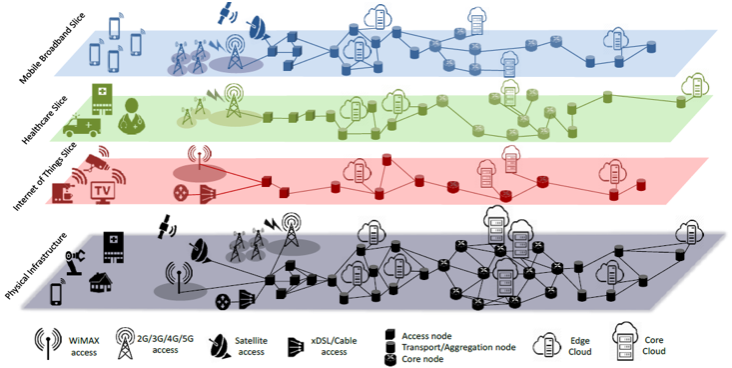
\includegraphics[width=.9\textwidth]{templates/images/chapter02/nw-slices.png}
    \caption{Network Slices on a Common Underlying Network. Source: \cite{OrdonezLucena2017NetworkSF}}
    \label{fig:nw-slices}
\end{figure}

The possibility to create on demand and in a programmable fashion, cost-efficient E2E network slices and dedicate them for the dynamic provisioning of diverse services is seen as a vital feature of 5G. In this vein, efforts are ongoing towards developing a 5G mobile system capable of deploying network slices of varying forms and sizes. Network slicing builds on top of the following seven main principles that shape the concept and related operations \cite{8320765}:

\begin{itemize}
    \item Automation: enables an on-demand configuration of network slicing without the need of fixed contractual agreements and manual intervention. 
    \item Isolation: is a fundamental property of network slicing that assures performance guarantees and security for each tenant even when different tenants use network slices for services with conflicting performance requirements.
    \item Customization: assures that the resources allocated to a particular tenant are efficiently utilized in order to meet the respective service requirements.
    \item Elasticity: is an essential feature related with the resources allocated to a particular network slice, in order to assure the desired \acrshort{sla} under varying resources and network conditions (e.g. the changes of network traffic or workload).
    \item Programmability: allows third parties to control the allocated slice resources (i.e. networking and cloud resources) via open \acrlong{api}s (APIs) that expose network capabilities facilitating on-demand service-oriented customization.
    \item End-to-end: is an inherent property of network slicing for facilitating a service delivery all the way from the service providers to the end-user. Such a property  stretches across different administrative domains and through that, unifies various network layers and heterogeneous technologies (e.g. \acrshort{ran}, core network, transport and cloud).
    \item Hierarchical abstraction: is a property of network slicing that has its roots on recursive virtualization, wherein the resource abstraction procedure is repeated on a hierarchical pattern with each successively higher level, offering a greater abstraction with a broader scope. In other words, the resources of a network slice, allocated to a particular tenant, can be further traded either partially or fully to yet another third  party. 
\end{itemize}

The network slicing process is broadly broken down into three main layers, namely the Service Instance layer, the \acrfull{nsi} layer, and the Resource layer. Each service instance reflects a service provided by a vertical segment, application provider or mobile network operator. The \acrshort{nsi} represents a set of resources customized to accommodate the performance requirements of a particular service and may contain none, one or a number of different sub-network instances. A sub-network instance can be a network function or a sub-set of network functions or resources realizing a part of an \acrshort{nsi}. 

\newpage

\acrshort{3gpp} refers to \acrlong{nssi} as \acrshort{nssi} and states that in order to be \acrshort{e2e}, an \acrshort{nsi} needs to consist of:

\begin{itemize}
    \item  \acrshort{nssi} \acrshort{ran}: an instance from a given (radio) access network slice subnet.
    
    A radio access network slice subnet consists of one or more \acrshort{ran} nodes (i.e. \acrshort{enb} nodes when using \acrshort{lte}, and \acrshort{gnb} nodes when using \acrshort{nr}), each embedding and delivering full radio access functionality to interact with the \acrshort{ue} over the radio interface. To introduce modularity and support for different deployment options, different initiatives has suggested the need to functionally split a \acrshort{ran} node into three types of units: \acrfull{ru}, \acrfull{du}, and \acrfull{cu}, briefly mentioned in Section \ref{chap:3gpp-rel15} as "\acrshort{ran} decomposition". For the most representative case, a \acrshort{ran} node may consist of a \acrshort{cu}, each serving one or more \acrshort{du}s, each in turn serving one or more \acrshort{ru}s.
   
    \item \acrshort{nssi} \acrfull{cn}: an instance from a given core network slice subnet. 
    
    A \acrshort{cn} slice subnet includes the functions from the \acrshort{3gpp} \acrshort{cn} that are in charge of providing connectivity between \acrshort{ran} nodes and the Data Network, as well as any other 3rd party \acrshort{af} providing value-added functionality.
    \item A Virtual Network providing connectivity within and across the two former \acrshort{nssi}s. 
    
    Focused on provided connectivity within the \acrshort{nsi} in an \acrshort{e2e} manner, the virtual network consists of a set of virtual links that may span across various network segments.
\end{itemize}

\acrshort{nssi}s resulting from the instantiation of the above-referred network slice subnets can be flexibly combined to provide different behaviors and performance levels, and hence different \acrshort{nsi}s.

%\newpage

\subsection{Roadmap of Network Slicing}
The implementation of network slicing needs to be gradual due to the evolution approach followed by the \acrshort{3gpp} 5G architecture in Rel. 15 and 16. Based on the network slicing roadmap proposed in \cite{4G_LTE_E2E-NS}, some of the most important phases expected are presented.

\begin{figure}[!ht]
    \centering
    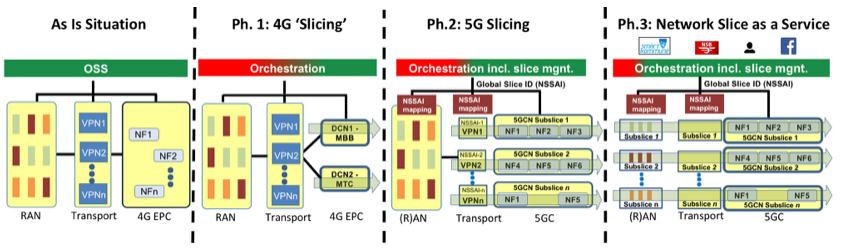
\includegraphics[width=.9\textwidth]{templates/images/chapter02/nw-slicing-roadmap.png}
    \caption{Roadmap of Network Slicing. Source: \cite{4G_LTE_E2E-NS}}
    \label{fig:nw-slicing-roadmap}
\end{figure}

"As-Is Situation" represents the current scenario where no network slicing and a single core network instance are present. In this scenario, \acrshort{qos} differentiation is offered at the Bearer level and \acrlong{apn}s (\acrshort{apn}s) are used for traffic separation while some form of isolation is implemented via a \acrfull{vpn}. Traffic can be separated for different customers but \acrshort{e2e} \acrfull{qos}, provisioning and the flexibility to have tailored network for vertical use cases cannot be implemented in an efficient manner.

Phase 1 is referred as  "4G Slicing" which  allows some level of traffic separation for overload mitigation and operational flexibility independent of other traffic.

Phase 2 will reference the specifications provided by the 3GPP Release 15 \acrfull{sa}, whose general concepts are outlined in Section \ref{chap:3gpp-rel15}. This phase is denominated as “5G Slicing” and consists of 5GCore. \acrshort{ran} and Transport layers support slicing via \acrfull{nssai}, with the latter leveraging \acrshort{vpn}s, each mapped according to said \acrshort{nssai}. Orchestration includes slice management but is not fully automated.

Phase 3 is labelled "\acrlong{nsaas}" (\acrshort{nsaas}) and is characterised by a fully automated network slicing operation. Unlike Phase 1 and 2 in which \acrshort{ran} and transport are not sliced, this phase involves slicing of the \acrshort{ran} and TN. In addition, it is expected to be able to host 3rd party \acrshort{nf}s, which enables new business opportunities.


\section{Network Slicing Types}

The \acrfull{itu} \cite{m.2083-0-201509} and \acrfull{5gppp} \cite{view_5g_architecture} have identified three broad use case families: enhanced mobile broadband, massive machine-type communications, and critical communications. Differences between these use cases amount to a set of heterogeneous and often contradictory requirements that cannot be satisfied by a one-size fits-all architecture. Diverse use cases need to be mapped to suitably tailored network structures. With this in mind, the architectural proposals for 5G aim to accommodate these use cases. The following sections describe how network slicing may utilise resources in order to serve these main use cases, while simultaneously respecting their requirements.

    \subsection{\acrfull{embb}}
    
    \acrshort{embb} is a set of services characterized by their need for high capacity links. This service type aims at supporting performance requirements of high data rates and high traffic densities. It is expected that the mobile capacity should increase 100 times over the capacity offered by current state of the art 4G systems to meet these requirements in urban user densities. Users should be able to achieve high speeds even at challenging scenarios such as on-the-go content streaming, while being at the cell edge and in crowded areas. In order to deliver NSaaS that provides this service, the \acrshort{csp} will place an emphasis on providing specific performance guarantees for \acrshort{kpi}s in the following areas: bandwidth, throughput, coverage and stability of connection.
    
    Some \acrshort{embb} services/applications will put more stress on the network from a \acrfull{up} traffic capacity point of view than others and thereby are more interesting from a Packet Core capacity perspective. This mandates specifying characteristics based on the need of each \acrshort{embb} service, Table \ref{tab:embb-sc-per} \cite{3GPP_TS_22.261} describes the performance requirements for high data rate and traffic density scenarios defined by 3GPP SA1 \cite{rel-15}.
    Depending upon the transmission delay, there is consideration on distributing User Plane on the Access Layer while hosting the rest of the functions centrally.

    \begin{sidewaystable*}
    \begin{threeparttable}
    \scriptsize
        \caption{\acrshort{embb} Scenarios and Requirements Identified by 3GPP}
        \label{tab:embb-sc-per}
    \begin{tabularx}{\textwidth}{@{}l*{10}{C}c@{}}
    \addlinespace
    %\addlinespace
    \toprule
        \multirow{2}{*}{Scenario} & \multicolumn{2}{c}{Experienced data rate} & \multicolumn{2}{c}{Area traffic capacity} & \multirow{2}{*}{User density} & \multirow{2}{*}{Activity factor} & \multirow{2}{*}{UE speed} & \multirow{2}{*}{Coverage} \\ 
        \cmidrule(r){2-3}\cmidrule(r){4-5}
        & Download & Upload & Download & Upload &  &  &  &  \\
    \addlinespace
    \midrule
    \addlinespace 
        Urban macro & 50 Mbps & 25 Mbps & 100 Gbps/km\textsuperscript{2} \tnote{4} & 50 Gbps/km\textsuperscript{2} \tnote{4} & 10 000/km\textsuperscript{2} & 20\% & Pedestrians and users in vehicles (up to 120 km/h & Full network \tnote{1} \\
        Rural macro & 50 Mbps & 25 Mbps & 1 Gbps/km\textsuperscript{2} \tnote{4} & 500 Gbps/km\textsuperscript{2} \tnote{4} & 100/km\textsuperscript{2} & 20\% & Pedestrians and users in vehicles (up to 120 km/h & Full network \tnote{1} \\
        Indoor hotspot & 1 Gbps & 500 Mbps & 15 Tbps/km\textsuperscript{2} & 2 Tbps/km\textsuperscript{2} & 250 000/km\textsuperscript{2} & \tnote{2} & Pedestrians & Office and residential \tnote{1} \tnote{3} \\
        Broadband access in a crowd & 25 Mbps & 50 Mbps & 3.75 Tbps/km\textsuperscript{2} & 7.5 Tbps/km\textsuperscript{2} & 500 000/km\textsuperscript{2} & 30\% & Pedestrians & Confined area \\
        Dense urban & 300 Mbps & 50 Mbps & 750 Gbps/km\textsuperscript{2} & 125 Gbps/km\textsuperscript{2} & 25 000/km\textsuperscript{2} & 10\% & Pedestrians and users in vehicles (up to 60 km/h) & Downtown \tnote{1} \\
        Broadcast-like services & Maximum 200 Mbps (per TV channel) & N/A & N/A & N/A & [15] TV channels of [20 Mbps] on one carrier & N/A & Pedestrians and users in vehicles (up to 500 km/h) & Full network \tnote{1} \\
        High-speed train & 50 Mbps & 25 Mbps & 15 Gbps/train & 7.5 Gbps/train & 1 000/train & 30\% & Users in trains (up to 500 km/h) & Along railways \tnote{1} \\
    \addlinespace 
    \midrule
    \end{tabularx}
    \begin{tablenotes}
        \RaggedRight
        \item[1] For users in vehicles, the UE can be connected to the network directly, or via an on-board moving base station.
        \item[2] A certain traffic mix is assumed; only some users use services that require the highest data rates [2].
        \item[3] For interactive audio and video services, for example, virtual meetings, the required two-way end-to-end latency (UL and DL) is 24 ms while the corresponding experienced data rate needs to be up to 8K 3D video [300 Mbps] in uplink and downlink.
        \item[4] These values are derived based on overall user density. Detailed information can be found in [10].
    \end{tablenotes}

    \end{threeparttable}
    \end{sidewaystable*}

    \subsection{\acrfull{urllc}}
    
    \acrshort{urllc} is a set of services with strict latency and reliability requirements. Basically, this service type aims at supporting performance requirements of low-latency and high-reliability while maintaining availability. Reliability increase can be achieved by dedicating appropriate resources to signalling, higher redundancy encoding and retransmissions. The above results in increased latency, proportional to packet size. If bandwidth requirements are low, by reducing packet size, low latency and high reliability simultaneously can be achieved, while reducing transmission times. 
    
    In order to guarantee the service is delivered at the required performance target, the \acrshort{csp} needs to prioritise resources to the \acrshort{urllc} slice, especially for mission-critical applications. It also needs to dynamically scale slices in the case of possible service degradation and may achieve high reliability by redundant transmission in the User Plane. 
    \acrshort{urllc} slices will provided by \acrshort{csp} for real-time control and feedback for the customer.
    
    From a communications perspective, two factors are of upmost importance and shall impact the definition of \acrshort{urllc} slice architecture in each Facility Site:
    
    \begin{enumerate}
        \item Latency: Sub-10ms \acrshort{e2e} latency is required for all use cases that can be mapped to the \acrshort{urllc} network slice. Note that many of the applications would require even sub-5ms latency, as seen on Table \ref{tab:urllc-sc-per}. 
        \item Reliability: The reliability is specified by the failure probability of packets (packet error rate) which are not successfully delivered to the receiver within the latency bound, as they are either erroneous, lost or arrive too late.
    \end{enumerate}
        
    \begin{sidewaystable*}
    \begin{threeparttable}
    \scriptsize
        \caption{\acrshort{urllc} Scenarios and Performance Identified by 3GPP}
        \label{tab:urllc-sc-per}
    \begin{tabularx}{\textwidth}{@{}l*{10}{C}c@{}}
    \addlinespace
    %\addlinespace
    \toprule
        Scenario & Max. allowed latency\tnote{2} & Survival time & Service availability\tnote{3} & Reliability\tnote{3} & User experienced data rate & Payload size\tnote{4} & Traffic density\tnote{5} & Connection density\tnote{6} & Service Area dimension\tnote{7} \\
    \addlinespace
    \midrule
    \addlinespace 
        Discrete automation & 10 ms & 0 ms & 99.99\% & 99.99\% & 10 Mbps & Small to big & 1 Tbps/km\textsuperscript{2} & 100 000 km\textsuperscript{2} & 1000 x 1000 x 30 m \\
        Process automation - remote control & 60 ms & 100 ms & 99.9999\% & 99.9999\% & 1 to 100 Mbps & Small to big & 100 Gbps/km\textsuperscript{2} & 1 000/km\textsuperscript{2} & 300 x 300 x 50 m \\
        Process automation - monitoring & 40 ms & 100 ms & 99.9\% & 99.9\% & 1 Mbps & Small & 10 Gbps/km\textsuperscript{2} & 10 000/km\textsuperscript{2} & 300 x 300 x 50 m \\
        Electricity distribution - medium voltage & 40 ms & 25 ms & 99.9\% & 99.9\% & 10 Mbps & Small to big & 10 Gbps/km\textsuperscript{2} & 1 000/km\textsuperscript{2} & 100 km along power line \\
        Electricity distribution - high voltage & 5 ms & 10 ms & 99.9999\% & 99.9999\% & 10 Mbps & Small & 100 Gbps/km\textsuperscript{2} & 1 000/km\textsuperscript{2} & 200 km along power line \\
        Intelligent transport systems & 30 ms & 100 ms & 99.9999\% & 99.9999\% & 10 Mbps & Small to big & 10 Gbps/km\textsuperscript{2} & 1 000/km\textsuperscript{2} & 2 km along road \\
    \addlinespace 
    \midrule
    \end{tabularx}
    \begin{tablenotes}
        \RaggedRight
        \item[1] Currently realised via wired communication lines. 
        \item[2] This is the maximum end-to-end latency allowed for the 5G system to deliver the service in the case the end-to-end latency is completely allocated to the 5G system from the UE to the Interface to Data Network.
        \item[3] Communication service availability relates to the service interfaces, and reliability relates to a given system entity. One or more retransmissions of network layer packets may take place in order to satisfy the reliability requirement.
        \item[4] Small: payload typically (<=) 256 bytes.
        \item[5] Based on the assumption that all connected applications within the service volume require the user experienced data rate.
        \item[6]  Under the assumption of 100\% 5G penetration.
        \item[7] Estimates of maximum dimensions; the last figure is the vertical dimension.
        \item[8] In dense urban areas.
        \item[9] All the values in this table are example values and not strict requirements. Deployment configurations should be taken into account when considering service offerings that meet the targets.
    \end{tablenotes}

    \end{threeparttable}
    \end{sidewaystable*}

\newpage
    
    \subsection{\acrfull{miot}}
    Heterogeneous access allows \acrshort{iot} devices to connect using whatever radio or fixed connectivity is available from both the device and the network. 5G-\acrshort{nr} utilizes spectrum bands for both low and very high bandwidth, as well as co-existence with cellular and non-cellular access networks but also other un-licensed radios. The operator is thus required to create and maintain the various instantiated \acrshort{iot} slices to offer services and enable the following scenarios:
    
    \begin{itemize}
        \item Enable individual needs of an \acrshort{iot} slice in terms of bandwidth, latency.
        \item Distribute efficiently resources of network slices involving resources at the Edge. Operators can offer resources and services at the edge of the network for \acrshort{iot} vendors to deploy (virtualised) applications and store collected data.
        \item Enable \acrshort{iot} Vendors to become “virtual operators” and build their own virtual network on top of a mobile operator and manage resources and services across a 5G network.
    \end{itemize}
    %added
    The \acrshort{miot} service type aims at supporting performance requirements of large number and high density of \acrshort{iot} devices. Some key aspects of these devices are their fully automated nature and the minimal interaction with humans, sending small amounts of information to the cloud. Some of these \acrshort{iot} devices are expected to be installed in remote, hard to access locations with bad coverage. Thus, a key requirement is the ability to use of very robust modulation and coding schemes. Median battery life is around a decade and the overall device cost should be low. Finally, their number is expected to explode in the coming years, thus base stations should be able to handle the additional overhead in signalling. In order to deliver NSaaS that provides this service, the \acrshort{csp} will place an emphasis on providing specific performance guarantees for \acrshort{kpi}s such as connection density (1,000,000 devices per km\textsuperscript{2}) and coverage (95\%) [55] while also guaranteeing security of the slice. Consumer privacy and security of the information proves of extreme importance for this type of service. 
    %eddad

\section{Network Slicing Requirements}
E2E network slicing inevitably adds an additional degree of complexity in the ecosystem, where each operator needs to deploy network slices internally and also facilitate the E2E deployment across several facility sites. Following there is a list of initial network slice requirements to be considered:

\begin{itemize}
    \item Orchestration: Slice-based services will require, not only the deployment across several administrative and operational domains, but also the integration of different technology domains. Their E2E nature requires orchestration of different computing and transport technologies.
    \item Operation: Each slice must behave as a dedicated network while sharing underlying resources, physical and virtual. Mechanisms need to be defined in order to abstract each customer slice.
    \item Scalability: The application of different \acrlong{sla} (SLAs) on the offered capabilities of management, control and customization of slices will directly impact scalability. Different levels depend on whether a network slice is inter or an intra-site.
    \item Service layer: The interaction with the vertical customers has an important requirement in the definition of the proper abstraction and templates to have a consistent service portfolio supported by different slice classes.
    \item Security and Isolation: Different network slices will be sharing the same infrastructure. The main requirement from the  \acrfull{iaas} and \acrfull{paas} is logical isolation of slices via appropriate networking, security grouping and multi tenancy implementation.
\end{itemize}

\newpage

\subsection{Network Slicing Use Cases}
    5G systems will support a wide range of use cases to vertical industries and their applications that wish to take advantage of their capabilities. These use cases will be supported by communication service providers (CSPs) who may offer \acrfull{nsaas} as a means of delivery. \acrshort{nsaas} is where the \acrshort{csp} offers network slices to their customers directly, rather than simply using slicing as an underlying capability to support other communication services. Each \acrshort{nsaas} will have a service description and \acrshort{sla} which will define the nature of the interaction between the \acrshort{csp} and said consumer.
    Slice providers and consumers can be described in terms of the business models between them and may fall into one of the following four categories:
    \begin{itemize}
    \item B2B (Business to Business): in which the \acrshort{csp} provides service to another business entity.
    \item B2C (Business to Consumer): in which the \acrshort{csp} providers service to an individual user.
    \item B2H (Business to household): in which the \acrshort{csp} provides service to a collection of individual users who form a single household and thus have some common characteristics.
    \item B2B2X (Business to Business to Everything): in which the \acrshort{csp} provides service to other business (such as other CSPs) who then offer a further service to their customers. 
    \end{itemize}
    From an architecture perspective, these four business models utilise one of two arrangements for the way in which the provider integrates their capabilities in order to deliver the end service.

\newpage

\section{Isolation on Network Slicing}
The use of a single, shared multi-domain network infrastructure makes isolation a key requirement in supporting network slicing. Isolation across \acrshort{nsi}s ensures that congestion, failures, attacks and lifecycle-related events (e.g. scaling in/out) of one \acrshort{nsi} does not negatively impact other \acrshort{nsi}s. Isolation is a broad concept embracing many dimensions, and will be studied from three main perspectives: performance, management and security. 

As previously mentioned, 5G network infrastructure is built out of a set of radio, computing, storage, and connectivity resources that can be flexibly combined to set up different \acrshort{nsi}s. These resources can be arranged into three main resource domains:

\begin{itemize}
    \item Radio Resource domain: consists of one or more antennas hosting RU functionality. A given antenna handles the operation of one or more cells, each assigned with specific radio resources to serve the \acrshort{ue} that are within the coverage area. These radio resources include multiple \acrfull{rf} carriers distributed across one or more spectrum bands which are consisted of several sub-carriers arranged into time-frequency resource grids known as \acrfull{prb}.
    \item \acrfull{dc} domain: consists of all the computing, storage, and networking resources that are defined within a \acrshort{dc}. Some are bundled together in physical, purpose-built devices ready to host \acrshort{pnf} instances, while others can be logically partitioned with the help of an abstraction layer. It is possible to have geographically distributed hierarchies, including edge and central \acrshort{dc}s. 
    \item \acrfull{tn} resource domain: consists of multiple physical \acrshort{tn} links providing connectivity throughout the entire hierarchical network infrastructure. These links can be similarly abstracted and partitioned, resulting in virtual links. Some of the \acrshort{tn} links will be defined within each administrative domain, providing connectivity between \acrshort{ran} nodes and \acrshort{dc}s, while others span across different domains, connecting central \acrshort{dc}s from different Facility Sites.
\end{itemize}

The resource (i.e. Radio, \acrshort{dc} and \acrshort{tn}) and management domains (i.e. 5G-\acrshort{ran} Controller, 5G-Core Controller, Transport controller, \acrshort{nfv}-\acrshort{mano}, and the \acrshort{e2e} Services Operations and Management) present the impact the three isolation dimensions have, without considering the presence of administrative domains. This means that the resource and management domains could be from the same or different sites.

    \subsubsection{Isolation in terms of Performance} 
    \label{chap:isolation-performance}
    
    Performance isolation in the network slicing context means that service-specific performance requirements are always satisfied on each \acrshort{nsi}, regardless of the congestions and workloads of other \acrshort{nsi}s running parallel. The level of performance committed for a \acrshort{nsi} needs to be assured in an \acrshort{e2e} manner (i.e. from the UE to the data center where the last \acrshort{nsi} component is allocated), across all the \acrshort{nssi}s that take part in the \acrshort{nsi}, including the connectivity between them. 
    \begin{enumerate}
        \item{Radio Resource Domain}
        
        Different \acrshort{nssi}s may share the limited set of radio resources available, mandating the definition of isolation mechanisms if performance isolation is desirable among \acrshort{nsi}s. This sharing is motivated by the fact that \acrshort{nssi}s are served within the same coverage area of a given antenna, and hence need to make a shared usage of the radio resources operated by this antenna. The isolation mechanisms vary depending on the scenario considered and include traffic isolation (i.e. avoid situations when traffic overload in one \acrshort{nssi} negatively affects the behavior of the rest of \acrshort{nssi}s) and electrical isolation (i.e. avoid mutual interference at the radio interface between the transmissions of different \acrshort{nssi}s) \cite{7891795}].
        Spectrum planning is the one that has the highest level of maturity, and hence can be seen as a feasible solution to be adopted for \acrshort{3gpp}'s Network Slicing Architecture.

\newpage

        \item{Datacenter Resource Domain} 
        
        \acrshort{dc}s include physical hardware that can be used to accommodate the \acrshort{nf}s of the different \acrshort{nsi}s. These \acrshort{nf}s can be either from the access part (\acrshort{an} \acrshort{nssi}s), or from the core part (CN \acrshort{nssi}s). The physical hardware of a \acrshort{dc} include both commodity and purpose-built hardware, while the latter can be seen as \acrshort{pnf} instances. Virtual resources result from the abstraction of the underlying commodity hardware, including computing, storage, and network equipment. The fact that \acrshort{vdu}s run on a common substrate brings potential risks on performance isolation, as failure or workload increase in one \acrshort{vdu} may decrease the performance of the rest of \acrshort{vdu}s sharing the same substrate. In virtualized environments, two approaches can be followed for \acrshort{vdu} hosting instantiation: 
        
        \begin{itemize}
        \item \acrshort{vnf} Instances from Different \acrshort{nsi}s on Separate Hardware Nodes.
        
        The first approach provides the most isolated environments for \acrshort{vdu} execution, as performance decrease and hardware failures in one node only affect the \acrshort{vdu} this node accommodates and not the rest of \acrshort{vdu}s. For the most critical \acrshort{nsi}s, compute nodes can be located in a dedicated availability zone, separated from any other zones in the \acrshort{dc}. Although allocating \acrshort{vdu}s from different \acrshort{nsi}s in different hardware nodes means achieving very great level of isolation among them, this approach commands high resource and energy usage.
        
        \item \acrshort{vnf} Instances from Different \acrshort{nsi}s Executed on a Shared Compute Node.
        
        The second approach allows for a more effective resource usage and energy efficiency, at the cost of providing less isolated environments for \acrshort{vdu} execution. Unlike the first approach, hardware failures and decreases of performance in one node may affect all the \acrshort{vdu}s running on this node.
        \end{itemize}

\newpage

        The introduction of server virtualization allows definition of \acrshort{vdu}s on top of the same compute node, providing them with separated execution environments. The isolation that each execution environment provides depends on the type of virtualization technology used. Currently, four types of virtualization technologies are available, each with different implications on the security ring-model as depicted in Figure \ref{fig:comparison-virtualization}. 
        
        \begin{figure}[!ht]
            \centering
            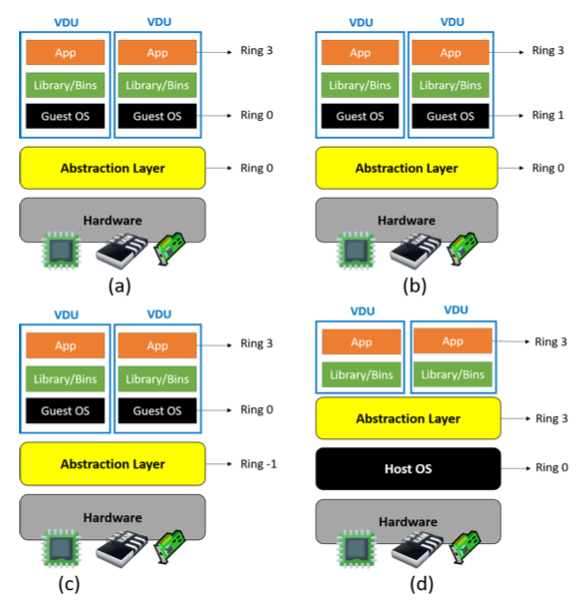
\includegraphics[width=0.75\textwidth]{templates/images/chapter02/comparison-virtualization.png}
            \caption[Comparison of Server Virtualization Technologies]{: (a) Para Virtualization, (b) Full Virtualization, (c) Full Virtualization with Hardware Assist\protect\footnotemark and (d) \acrshort{os} Virtualization. Source: \cite{adrian_gallego_2019_2668763}}
            \label{fig:comparison-virtualization}
        \end{figure}

\footnotetext{Note that full virtualization technologies with hardware assist (i.e. Intel VT and AMD-V) introduces a more privileged ring level (ring -1) to the original x86 ring model. In this new ring level, the abstraction layer uses processor extension to intercept and emulate privilege instructions, leaving ring 0 available for \acrshort{vdu}s, whereas this would be reserved by the operating system's kernel.}

        As result of the application of the four above-referred technologies, two types of \acrshort{vdu}s are outlined: \acrshort{vdu}s with their own guest \acrshort{os} and \acrshort{vdu}s sharing the same host \acrshort{os} as depicted in Figure \ref{fig:vm-unikernel-container}. 
        
        Those result in two types of abstraction layer being identified:
        \begin{itemize}
            \item Hypervisor: applicable to para virtualization, full virtualization, and full virtualization with hardware assist. This abstraction layer allows the definition of \acrshort{vdu}s, each with its guest \acrshort{os}. The \acrshort{vdu}s resulting from the hypervisor are traditional \acrlong{vm}s (VMs). However, in recent years, a new type of \acrshort{vdu}, named "unikernel", resembles a \acrshort{vm} but is built with a lightweight and specialized guest \acrshort{os}. Unlike \acrshort{vm}s, a unikernel can only run a single process, and cannot benefit from full virtualization with hardware assist, as it contains only aboslutely necessary components to run a specific application.
            \item Container engine: applicable to \acrshort{os} virtualization, this abstraction layer allows the definition of \acrshort{vdu}s running on top of the same \acrshort{os}, without the possibility to host their own. These \acrshort{vdu}s resulting from the abstraction carried out by container engine are referred to as containers.
        \end{itemize}

        \begin{figure}[!ht]
            \centering
            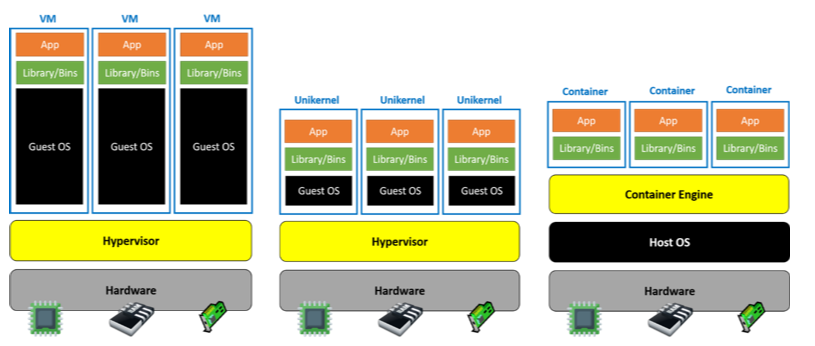
\includegraphics[width=.9\textwidth]{templates/images/chapter02/vm-unikernel-container.png}
            \caption{\acrshort{vm}s vs Unikernels vs Containers in Terms of Isolation. Source: \cite{adrian_gallego_2019_2668763}}
            \label{fig:vm-unikernel-container}
        \end{figure}
        
        \begin{table}[!ht]
           \begin{threeparttable}
        \caption[Comparison Between Types of \acrshort{vdu}s]{on Top of which \acrshort{vnf} Instances Run}
        \label{tab:vdus}
        \setlength\tabcolsep{1pt} % make LaTeX figure out intercolumn spacing
        
        \begin{tabular*}{\columnwidth}{@{\extracolsep{\fill}} lllll}
        \toprule
             \acrshort{vdu} Type &Ring Level &Isolation provider &Image size &Operation agility \\
        %     \multicolumn{4}{c}{Accuracy (\%)} \\ 
        %\cmidrule{3-6}
        %     & & K3 & K6 & L1 & mean\tnote{c} \\
        \midrule
              \textbf{\acrshort{vm}} &Level 0 or -1 &Hypervisor &Large &Low \\
        \addlinespace
             \textbf{Unikernel} &Level 0 &Hypervisor & Small & Medium \\
        \addlinespace
              \textbf{Container} &Level 3 enforced at Level 0 &Host \acrshort{os} &Medium &High\\
        \bottomrule
        \end{tabular*}
        
        \smallskip
        \scriptsize
           \end{threeparttable}
        \end{table}
        
        As seen from Table 5.2, the most isolated environment is provided with a \acrshort{vm} at the cost of less speed of operation, followed by the unikernel that provides more agility and reduced image size. Containers provided the least degree of isolation, although they allow for great agility in run-time operations. The selection of each \acrshort{vdu} type for \acrshort{vnf} hosting depends on the necessity of the \acrshort{vnf} operation, and the degree of isolation required. The use of separate physical appliances and \acrshort{vm}s are known to be matured solutions for providing isolation in the \acrshort{dc} resource domain. Unikernels, although bringing some benefits compared to \acrshort{vm}s, need to reach more maturity and popularity before considering them as firm candidates to replace \acrshort{vm}s. Finally, containerization technology is gaining some maturity in the last years, empowered by the adoption of Service Based Architecture (SBA) for \acrshort{3gpp}’s 5GC. The adoption of this solution is expected for \acrshort{3gpp} Rel. 15 and 16 SA.

        \item{\acrfull{tn} Resource Domain}
        
        Virtual links resulting from the abstraction of the underlying \acrshort{tn} links can be arranged into virtual networks, each providing intra-\acrshort{nsi} connectivity (i.e. connectivity across P/\acrshort{vnf} instances from the \acrshort{nssi} \acrshort{ran} and \acrshort{nssi} CN) with performance guarantee. Both wired and wireless \acrshort{tn} technologies can be used, with the former including optical and gray optics, whereas the latter encompasses both wireless (i.e. packet microwave and mm-wave) and satellite solutions as Physical Layer (L1) technologies. 
        It is to be expected that, in some cases, the common \acrshort{tn} infrastructure will be shared between multiple 5G services. Network slicing isolation is thereby achieved by the introduction of some form of encapsulation, for the differentiation of virtual links operating on top of a shared substrate and the selection of corresponding Layer technologies towards the realization of these virtual networks. The introduction of encapsulation enables different virtual networks to be deployed on top of physical links that compose the underlying \acrshort{tn} infrastructure, differentiated by the degree of isolation they provide.
        
        Soft isolation is implemented by statistically multiplexing the traffic from two or more VNs onto a common circuit switched connection using a packet technology (e.g., Ethernet \acrfull{vlan}, \acrfull{mpls} tunnel). Isolation is enforced at the packet layer, permitting sharing of resources across different virtual links, since resources are only dedicated on a temporary basis. This allows greater statistical multiplexing on network resources in different links and leads to better economy at the cost of opening up the possibility to suffer from congestion in the network, in all the virtual links making use of those resources.
        
        Hard isolation is implemented by providing independent circuit switched connections for the exclusive use of one VN (e.g. Time Division Multiplexing (TDM) based approaches, assignment of different fibre cables etc.). Hard isolation solutions allow reaching high degree of isolation between virtual links, at the expense of allocating dedicated resources on a long term and end-to-end basis. This means that that the full cost of the resources must be borne by the \acrshort{nsi} whose VL is allocated with those resources.   
\end{enumerate}
    
    \subsubsection{Isolation in terms of Management and Orchestration}
    \label{chap:isolation-mano}
    Isolation at the \acrshort{mano} level assumes the existence of tenants at the orchestration level (e.g., Multitenancy in \acrshort{osm}, ONAP). Each tenant has an exclusive view and management of specific \acrshort{vnf}s, NSs and the isolated resources at the \acrshort{ran}, Core and TN, enabling the management and orchestration of a particular slice. A default master tenant usually called “administrator”, is in charge of the management and orchestration of all slices and the physical and logical resources that comprise them.  Multitenancy at the \acrshort{vim} level articulates the isolation mechanisms defined in compute, storage and tenant networks, allowing for a tenant to only see and administrate the resources that are assigned to it.
    One important concept is the shared part. It is important to employ the isolation mechanisms mentioned in previous sections (e.g. \acrshort{ran} slicing at the carrier and \acrshort{prb} level, transport slicing at the wavelength, time slot, logical bandwidth level). From previous sections, it is apparent that shared resources is a critical part of operation. As to be expected, isolation cannot be guaranteed in all cases (i.e. when sharing same antenna, cable and compute node across multiple slices). Tenants may demand isolation of resources allocated to management regarding isolation of compute and storage resources. This makes it possible to obtain all properties of virtualized computing systems, as mentioned in the previous section, enabling tenants with different levels of isolation at the management level.

    \subsubsection{Isolation in terms of Security}
    \label{chap:isolation-security}
    Security as a term, encompasses different aspects in the provisioning, operation and use of any network services. For that reason, slices must adhere to general security properties, based on the three dimensions of a network service. These dimensions have obvious implications to slice isolation and namely are:
    
    \begin{itemize}
        \item Protection: in what implies that a service is immune to attacks from any adversary attempting to distort in any means its functionality or features. Isolation in terms of protection ensures each slice is immune from attacks on other slices or parts of the external network.
        
        \item Privacy: requiring that no data from any actor in the service (provider, consumer, end user) is accessed by unauthorized parties. Isolation in terms of privacy ensures each slice has adequate mechanisms to protect integrity and confidentiality and sensitive information (i.e. configuration, management, subscriber, and accounting information) from being accessed by other entities.
        
        \item Accountability: which translates into enforcing proper authentication, authorization and accounting, so no action is performed without verifying the identity, access rights and properly maintaining a record for further auditing.
    \end{itemize}
